% ==========================================
% CHAPTER 3: APPLICATION REQUIREMENTS
% ==========================================
\chapter{Application Requirements and System Architecture}
\label{chap:architecture}

This chapter connects the theoretical foundations from Chapter 2 with the actual implementation of KinetoCheck. It begins by turning the broad research goals and identified gaps into a concrete set of system requirements. From there, the modular architecture is introduced, breaking down the layered components and software design patterns that bring the platform to life. Together, this requirements-and-architecture blueprint sets the stage for the practical coding details and experimental results that follow.

\section{System Scope and Problem Definition}
KinetoCheck addresses the practical problem of evaluating rehabilitation exercise quality from user-provided videos, with automated feedback that is both machine-generated and interpretable. The application is designed for a semi-supervised usage scenario in which a user uploads a recording, the pipeline performs pose extraction and model inference, and the system returns a decision, score, and explanatory artifacts.

\section{System Requirements}
The system requirements are divided into functional and non-functional concerns so that the application goals and quality constraints remain explicit.

\subsection{Functional Requirements}
Functional requirements define what the application must do.
\begin{enumerate}
    \item \textbf{Video Upload:} The system shall accept a user-uploaded exercise video in supported formats: mp4, mov, mkv, avi, and webm.
    \item \textbf{Input Validation:} The system shall validate file type, file size, and basic integrity before processing.
    \item \textbf{Pose Extraction:} The system shall run MediaPipe Pose Landmarker to extract keypoints frame-by-frame from the uploaded video.
    \item \textbf{Preprocessing Consistency:} The extracted keypoints shall be transformed using the same preprocessing logic used during model training.
    \item \textbf{Inference Execution:} The system shall load the exercise-specific checkpoint and compute a similarity-based prediction.
    \item \textbf{Decision and Score Reporting:} The system shall return a predicted label (correct/incorrect), a score, and the threshold used for the decision.
    \item \textbf{Joint-Level Feedback:} The system shall identify and expose high-importance/problematic joints used for feedback visualization.
    \item \textbf{Annotated Output:} The system shall produce an annotated video or frame overlays that highlight key feedback regions.
    \item \textbf{Structured Report Export:} The system shall generate and store a JSON report containing core inference artifacts.
    \item \textbf{Analytics Summary:} The system shall generate user-level exercise statistics and overview metrics from inference outputs.
    \item \textbf{Asset Retrieval:} The web layer shall provide access to generated reports and media artifacts.
\end{enumerate}

\subsection{Non-Functional Requirements}
Non-functional requirements define quality attributes and operational constraints.
\begin{enumerate}
    \item \textbf{Reproducibility:} Given the same input and model version, the system should produce stable outputs within acceptable numerical tolerance.
    \item \textbf{Maintainability:} Training, inference, and web modules should remain separated to support independent updates.
    \item \textbf{Latency Expectation:} End-to-end processing time should be bounded for practical usability, with an acceptance target of processing time $\leq 1.0\times$ input video duration on target deployment hardware.
    \item \textbf{Robustness to Missing Detections:} The pipeline should handle partial landmark dropout through interpolation, masking, or safe fallback behavior.
    \item \textbf{Browser Compatibility:} The web layer targets the latest two stable versions of Chrome, Edge, Firefox, and Safari.
    \item \textbf{Traceability:} Each result should be linked to model version, threshold configuration, and processing timestamp.
    \item \textbf{Error Transparency:} Invalid inputs or failed processing stages should produce explicit and user-readable error messages.
    \item \textbf{Analytics Consistency:} Aggregated statistics should remain traceable to the underlying inference session, model version, and timestamp.
\end{enumerate}

The consolidated functional and non-functional requirements matrix is presented in Table~\ref{tab:T5}.


\begin{table}[H]
\centering
\small
\setlength{\tabcolsep}{4pt}
\renewcommand{\arraystretch}{1.12}
\begin{tabularx}{\textwidth}{|>{\centering\arraybackslash}p{1.2cm}|>{\centering\arraybackslash}p{0.9cm}|>{\raggedright\arraybackslash}X|>{\centering\arraybackslash}p{1.4cm}|>{\raggedright\arraybackslash}p{2.5cm}|>{\raggedright\arraybackslash}X|}
\hline
Req ID & Type & Requirement & Priority & Verification Method & Acceptance Criterion \\
\hline
F-01 & F & User shall upload a supported video file for analysis. & Must & Functional test & Valid file is accepted and processing starts. \\
F-02 & F & System shall extract 17-joint pose sequence from uploaded video. & Must & Pipeline log + output check & Sequence tensor generated with expected shape. \\
F-03 & F & System shall run checkpoint-based inference and output label/score. & Must & Functional test & Report contains predicted label, score, threshold. \\
F-04 & F & System shall generate an annotated output video. & Must & Artifact inspection & Annotated MP4 exists and is downloadable. \\
F-05 & F & System shall provide problematic-joint feedback in report. & Should & JSON schema check & worst\_joints field includes ranked entries. \\
NF-01 & NF & Pipeline shall be reproducible from scripts/configuration. & Must & Re-run reproducibility test & Comparable metrics reproduced from same checkpoint/data. \\
NF-02 & NF & System shall be maintainable with modular preprocessing/model/inference code. & Should & Code review & Clear module boundaries and documented interfaces. \\
NF-03 & NF & Inference shall tolerate temporary landmark dropouts. & Must & Robustness test & No crash; missing frames handled with fallback strategy. \\
NF-04 & NF & Web output shall be browser-compatible for video playback. & Should & Cross-browser test & Playable or downloadable output in major browsers. \\
\hline
\end{tabularx}
\caption{Functional and non-functional requirements matrix}
\label{tab:T5}
\end{table}

The requirements above define the boundaries for the implementation. The following architectural overview shows how the application components map onto those requirements.

\section{Architectural Overview}
KinetoCheck is organized as a modular pipeline that separates input acquisition, preprocessing, model inference, feedback generation, and reporting. This separation keeps the learning components independent from the application layer so that model variants can be evaluated without changing the user workflow.

\begin{figure}[H]
    \centering
    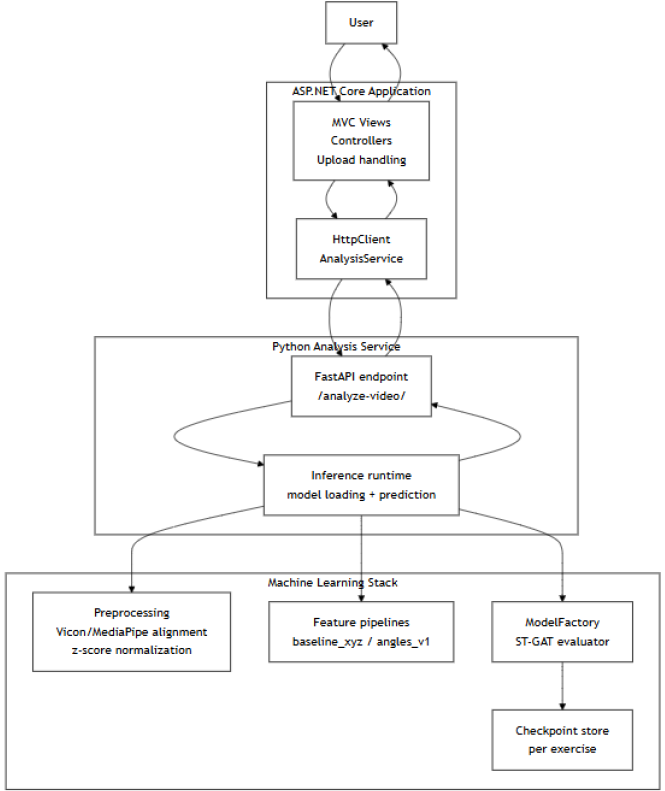
\includegraphics[width=0.9\textwidth]{figures/context_diagram.png}
    \caption{System Context Diagram depicting the separation of concerns between the presentation (ASP.NET), API (FastAPI), and machine learning layers.}
    \label{fig:system-context}
\end{figure}

The system can be summarized in five layers:
\begin{enumerate}
    \item \textbf{Input layer:} receives exercise videos, live camera streams, or dataset sequences.
    \item \textbf{Preprocessing layer:} extracts 17-joint pose sequences, aligns dataset formats, normalizes body coordinates, and constructs feature tensors.
    \item \textbf{Inference layer:} applies the ST-GAT encoder, optional phase alignment, optional frame-level decoding, and similarity scoring.
    \item \textbf{Output layer:} produces predictions, score values, and joint-level feedback for visualization.
    \item \textbf{Analytics layer:} aggregates repeated inference sessions into user-level statistics, exercise summaries, and trend reports.
\end{enumerate}

\subsection{Model and Inference Design}
The data pipeline must preserve compatibility between training and inference domains. Input video is transformed into a temporal sequence of 17-joint keypoints. The fixed tensor specification is: raw pose sequence as float32 with shape \texttt{(N, 17, 3)}, preprocessed sequence as float32 with shape \texttt{(120, 17, 3)}, and model input as float32 with shape \texttt{(B, C, 120, 17)}.

The final response package includes: prediction label and score; threshold and model identifier; problematic-joint list; annotated output media path; and JSON report path.

\begin{figure}[H]
    \centering
    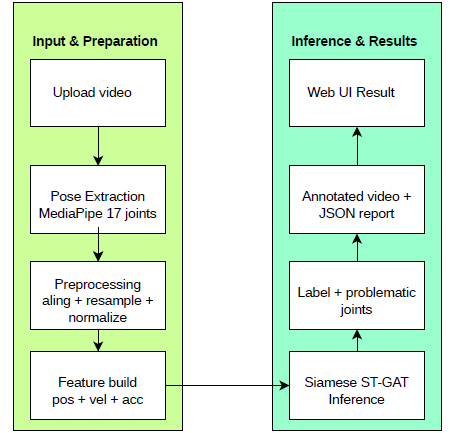
\includegraphics[width=0.6\textwidth]{figures/end-to-end.png}
    \caption{End-to-end input-output flow of the KinetoCheck application, from video upload to generated report and annotated media.}
    \label{fig:end-to-end-flow}
\end{figure}

\subsection{Data Flow and Artifact Specification}
Prediction is derived from a similarity score compared against an exercise-specific threshold. The thresholding policy must be versioned because it directly influences precision-recall behavior and user feedback interpretation. In the current implementation, threshold calibration sweeps 101 linearly spaced threshold candidates, selects the threshold that maximizes validation F1, and applies the decision rule: \texttt{correct if score >= threshold}.

To ensure reproducibility, the practical system documents the following elements:
\begin{itemize}
    \item train/validation/test partition policy (including Leave-One-Subject-Out (LOSO) if used);
    \item hyperparameter configuration and optimizer settings;
    \item checkpoint naming/versioning convention;
    \item per-exercise metrics and threshold logs;
    \item software dependencies and runtime environment.
\end{itemize}

\subsection{Analytics and Reporting Layer}
A dedicated analytics and reporting layer sits after inference and before long-term user-facing outputs. The purpose of this layer is to convert individual inference results into a longitudinal view of rehabilitation progress.

The analytics pipeline reuses existing inference artifacts instead of re-running the model. A typical session flow is:
\begin{enumerate}
    \item run exercise inference and store the score, threshold, label, and joint feedback;
    \item attach metadata such as exercise identifier, model version, and timestamp;
    \item aggregate repeated sessions by user, exercise, or time window;
    \item compute summary statistics and trend values;
    \item deliver the result to the dashboard or export it as JSON or CSV.
\end{enumerate}

\section{Software Design Patterns}

\subsection{Factory and Singleton Cache Patterns}
The factory pattern is used to create the correct evaluator implementation based on the selected checkpoint configuration. Loaded models are cached so that repeated inference requests do not reload weights from disk, reducing startup overhead.

\subsection{Composition and Component Isolation}
The phase aligner, frame decoder, and joint scorer are implemented as separate components. This keeps the architecture testable and makes it possible to improve one part of the system without rewriting the entire model stack.

This chapter has formalized both the practical requirements and the architectural design of KinetoCheck. By bridging specification and implementation design, it establishes the engineering baseline needed to interpret the training strategies and implementation details presented in the next chapter.